\documentclass[11pt,a4paper]{article}

%
% $Id: howtobuild.tex,v 1.14 2006/04/25 14:20:24 schnelle Exp $
%

\usepackage[latin1]{inputenc}
\usepackage{graphics}
\usepackage{graphicx}
\usepackage{url}
\usepackage{listings}
\usepackage{xcolor}
\usepackage{jvoicexml}
\usepackage[pdftex, citecolor=black, urlcolor=black,
linkcolor=black, colorlinks=black, colorlinks=true,
 bookmarksopen=true]{hyperref}
\include{version}

\title{How to build JVoiceXML \jvxmlversion}
\version{1.9.9}
\author{Dr. Dirk Schnelle-Walka}
\email{dirk.schnelle@jvoicexml.org}
\date{\today}

\begin{document}

\pagestyle{empty}
\lstset{language=Java,language=XML,
        backgroundcolor=\color{lightgray},
        basicstyle=\small,
        numbers=left,
        numberstyle=\tiny,
        breaklines=true, 
        breakatwhitespace=false, 
        flexiblecolumns,
        stepnumber=5}

\maketitle

\pagestyle{headings}

\tableofcontents

\newpage

\begin{abstract}
This documents describes the steps you have to perform, when you want
to build JVoiceXML or develop code for the JVoiceXML project. It gives
information about the requirements of your development environment 
and our coding conventions.
\end{abstract}

\section{Introduction}
\label{sec:introduction}

JVoiceXML is a free VoiceXML~\cite{w3.org:voicexml} implementation written in 
the JAVA programming language. It offers a library for easy VoiceXML
document creation and a VoiceXML interpreter to process 
VoiceXML documents using JAVA standard APIs such as JSAPI~\cite{sun:jsapi} and
JTAPI~\cite{sun:jsapi}.

VoiceXML is hosted at SourceForge~\cite{sourceforge} as an open source project.
You find everything that is related to this project under
\url{http://sourceforge.net/projects/jvoicexml/}.

This document refers to UNIX and Windows systems. JVoiceXML will work 
any other operating systems that support Java 6, too.

Nobody is perfect, so you may find some errors or small things to correct.
Please let me know if you think you found something that should be written
differently.

\section{Copyright}
\label{sec:copyright}

JVoiceXML uses the GNU library general public license~\cite{gnu:lgpg}. 
This is mentioned in all our source files as a unique header, see
section~\ref{sec:code-conventions}.
You can find a copy in the file COPYING in the \$\{JVOICEXML\_HOME\}
directory. This means that you are allowed to use JVoiceXML
library in your commercial programs. If you make some nice
enhancements it would be great, if you could send us your
modifications so that we can make it available to the public.

JVoiceXML is free software; you can redistribute it and/or
modify it under the terms of the GNU Library General Public
License as published by the Free Software Foundation; either
version 2 of the License, or (at your option) any later version.

JVoiceXML is distributed in the hope that it will be useful,
but WITHOUT ANY WARRANTY; without even the implied warranty of
MERCHANTABILITY or FITNESS FOR A PARTICULAR PURPOSE. See the GNU
Library General Public License for more details.

You should have received a copy of the GNU Library General Public
License along with this library; if not, write to the Free
Foundation, Inc., 59 Temple Place, Suite 330, Boston, MA  02111-1307  USA

\section{Download the Source Code}

\subsection{Download the source archive}

You can download a the source code for the available releases from 
\url{http://jvoicexml.sourceforge.net/downloads.html}. The source code is part of
the binary distribution and can be obtained by running the installer. This is
not the recommended way. Please use the SVN repository as described in
the following sections. \\

\subsection{SVN repository}
\label{sec:svn-repository}

If you want to stay at the current state of development you have to use
the SVN repository from Source Forge~\cite{sourceforge}.
This is also the preferred way.

This section describe the parameters to access the SVN repository 
using the command line. Feel free to grab the required parameters from
this description and feed your favorite tool with them.

\begin{lstlisting}
svn checkout --username=<your name> \
  https://svn.code.sf.net/p/jvoicexml/code/trunk jvoicexml
\end{lstlisting}

This will check out all projects of \texttt{trunk} of
into the folder \texttt{jvoicexml}. Please refer to
section~\ref{sec:jvoicexml-core} if you want to checkout
only a minimal set of projects. Here, the required projects
to build the core project are marked as \emph{required}.

Since all the third party libraries are checked a checkout may
take a while.

An alternative way is given by using svn+ssh. In this case code is checked out
by
\begin{lstlisting}
svn checkout --username=<your name>
  svn+ssh://<your name>@svn.code.sf.net/p/jvoicexml/code/trunk jvoicexml
\end{lstlisting}

For the eclipse users on Windows the following article might be of some interest
\url{http://www.woodwardweb.com/java/howto_configure.html}. 

A screenshot from a checkout in eclipse is shown in
figure~\ref{fig:eclipse-projects}.
\begin{figure}
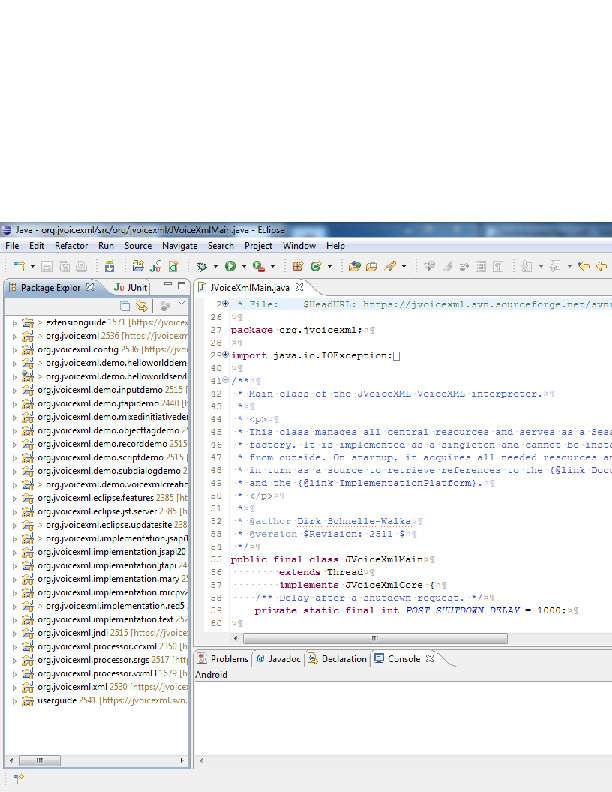
\includegraphics[width=\linewidth]{eclipse-projects.png}
\caption{Eclipse project overview of JVoiceXML}
\label{fig:eclipse-projects}
\end{figure}

\textbf{Note:} UNIX file and directory names are case sensitive.

All projects follow the convention that they have the same name as the jar
that will be produced when bundling them. For instance, the jar \lstinline{org.jvoicexml.xml.jar}
is built by the project \lstinline{org.jvoicexm.xml}.

An alternative way to download the contents of the repository is to use the 
nightly build system for that purpose. Download all jars from
\url{http://jvoicexml.svn.sourceforge.net/viewvc/jvoicexml/core/trunk/org.jvoicexml/3rdparty/svnant/lib/}
as well as the ANT file for the nightly build at
\url{http://jvoicexml.svn.sourceforge.net/viewvc/jvoicexml/core/trunk/org.jvoicexml/nightly.xml}
into the directory where you want to have all those project files. This may be
your eclipse workspace.

Then change in to that directory and run
\begin{lstlisting}
svn co \
ant -f nightly.xml checkout
\end{lstlisting}


\section{Required Software}
\label{sec:required-software}

Since JVoiceXML is written in JAVA you will at least need a
JAVA compiler, see section~\ref{sec:ide}, an editor or preferably a JAVA
IDE, see section~\ref{sec:ide}, and ANT, see section~\ref{sec:ant}, to build the
binaries. All used third party libraries can be downloaded from the CVS, SVN or
comparable repository or from their home pages. The file
\texttt{doc/libraries.xhtml} contains a list of all used libraries.


\subsection{IDE}
\label{sec:ide}

JVoiceXML is being developed using eclipse 4.2, but you can use the IDE of your
choice to edit the sources and compile the binaries. You can even use a simple
text editor to perform this job. Nevertheless there are some restriction that
you cannot work around.

Your IDE must support

\begin{itemize}
\item JavaSE 7
\item ANT 1.7
\end{itemize}

\subsection{JAVA}
\label{sec:java}

Parts of the code of JVoiceXML are using features from the JAVA 7 API, so that
you will need at least J2SE 7 to compile the code. You can download it
for free from \url{http://oracle.com/technetwork/java/javase/downloads/index.html}.


\subsubsection{Eclipse settings}
\label{sec:eclipse}

If you are not using eclipse as your favorite IDE, you may ignore this section.
We are using the \emph{Eclipse IDE for Java EE Developers} version 4.2 for
the development of JVoiceXML. The subversion repository contains the eclipse
project settings. This way, you there is no need to import the
project into eclipse. The project settings will be detected 
automatically when you checkout the projects. However you are requested to configure the execution
environment development for Java 7 \emph{JavaSE-1.7} to point to a valid JDK.
The use of execution environments makes the development independent of the
used version of the Java 7 SDK.

A screenshot for a possible configuration is shown in
figure~\ref{fig:eclipse-execution-environments}.
\begin{figure}
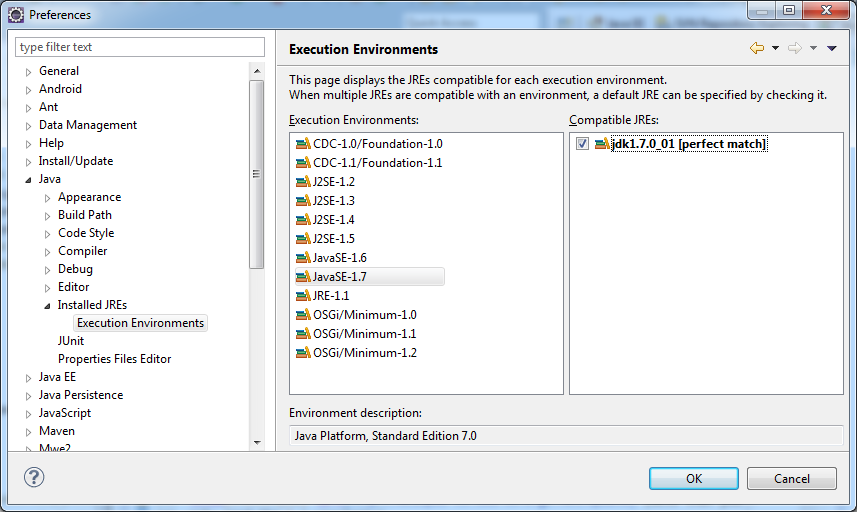
\includegraphics[width=\linewidth]{eclipse-execution-environments}
\caption{Configuration of the Java 7 Execution Environment in eclipse}
\label{fig:eclipse-execution-environments}
\end{figure}

Eclipse is configured to use the folder \texttt{eclipse-compiled} as output
since this may caus some interfernece with the ANT build
scripts\footnote{\url{https://bugs.eclipse.org/bugs/show_bug.cgi?id=210746}}.

\paragraph{Eclipse Plug-ins}

The development of JVoiceXML relies on some plug-ins that are not part of the
IDE. You will need to install the following eclipse plug-ins via the eclipse
Software Update mechanism.

Below is a list of the required update URLs.

\begin{description}
\item[Checkstyle] \url{http://eclipse-cs.sourceforge.net/update} (Note that you
only need the 5.x version)
\item[Subversion] \url{http://subclipse.tigris.org/update_1.6.x}
(Alternatively, you can also use subversive or a similar SVN client)
\item[TeXlipse] \url{http://texlipse.sourceforge.net} (optional if you want to
edit the documentation)
\item[Protocol Buffers Development Tools] \url{http://code.google.com/p/protobuf-dt/}
(optional if you want to edit the protobuf files in the sub project \texttt{org.jvoicexml.mmi.events})
\end{description}

\subsection{ANT}
\label{sec:ant}

JVoiceXML is being built by an ANT build file It is recommended that
you use at least ANT 1.7.0. 
If you don't have ANT installed, you can download the current release
from \url{http://ant.apache.org}. This should not be necessary if ANT is builtin
your IDE as it is the case with eclipse.

The build file allows you to override the settings by using a custom 
properties file jvoicexml.properties in the \$\{JVOICEXML\_HOME\}
directory.

Nearly all IDE's feature an ANT integration. This allows to use
your favorite IDE.

\subsubsection{ANT Support for Eclipse}
\label{sec:ant-eclipse}

The ANT project files are usually named \texttt{build.xml} and reside in
the folders of the subprojects. In order to run an ANT target from within
eclipse you can open these build files with the ANT editor as shown in
figure~\ref{fig:eclipse-open-ant-editor}.
\begin{figure}
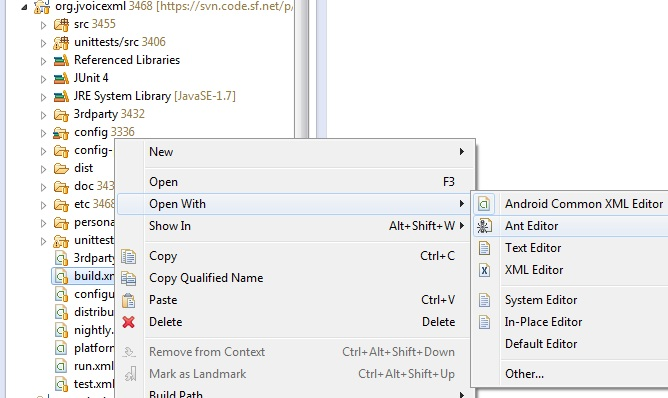
\includegraphics[width=\linewidth]{eclipse-open-ant-editor}
\caption{Open the ANT build file with the ANT editor}
\label{fig:eclipse-open-ant-editor}
\end{figure}
The targets that can be executed will be shown in eclipse's outline view.
Right-click the target to execute and select \emph{Run As} and the
\emph{ANT Build} as shown in figure~\ref{fig:eclipse-run-ant}.
\begin{figure}
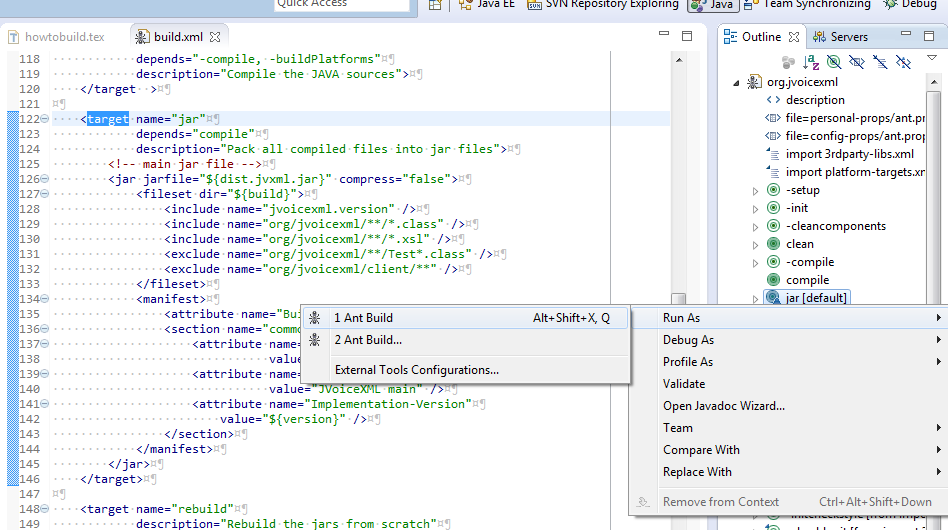
\includegraphics[width=\linewidth]{eclipse-run-ant}
\caption{Run an ANT target}
\label{fig:eclipse-run-ant}
\end{figure}
Afterwards, it may be necessary to refresh the project to synchronize generated
files with eclipse's view onto the file system.

Some more information for executing ANT targets from within eclipse are given at
the end of section~\ref{sec:ant-build-file}. 

Note: Please use the ANT build system. An attempt to run JVoiceXML from eclipse
directly may result in strange errors and a huge amount of adaptions to the
classpath.

\subsection{Tomcat}
\label{sec:tomcat}

For the system test and for some demos you will need to have a servlet
container installed. We use Tomcat 5.5 for that purpose. You can download this
release from \url{http://tomcat.apache.org}.

This is not needed if you do not use the servlet based demos or want to run the
system test.

\subsection{\LaTeX}

The documentation is being written using \LaTeX. If you want to edit the
documentation you will need to install a \LaTeX system like MiKTeX
\url{http://miktex.org} for windows or tetex on Linux systems.

This is not needed if you do not want to author the documentation or create a
distribution.

\section{Project Conventions}

JVoiceXML comprises several projects. Some of them are described in more
detail in the following section. All these projects follow some conventions
that should help to stay oriented.

The base namespace for all projects is \lstinline{org.jvoicexml}. Dependent 
projects may extend this namespace. For instance the namespace for the
XML library is \lstinline{org.jvoicexml.xml}.

The project names have the same name as the jar that they produce. This
makes it easier to find the project related to a specific Java archive.
For instance the project name for the XML library is
\lstinline{org.jvoicexml.xml}. It produces the jar
\texttt{org.jvoicexml.xml.jar}.
The drawback of this approach is that you will be confronted 
with a huge list of projects. The minimal set of projects
that are required to build JVoiceXML is marked in the list
given in section~\ref{sec:jvoicexml-core}.

The project names generally also reflect the overall architecture as shown in
figure~\ref{fig:main-components}.
\begin{figure}
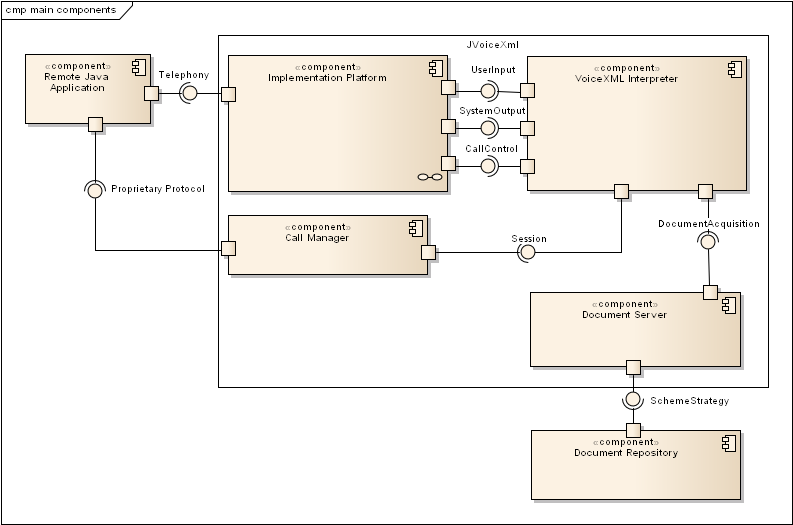
\includegraphics[width=\linewidth]{main-components.png}
\caption{JVoiceXML general architecture}
\label{fig:main-components}
\end{figure}
These components can be mapped to the packages as shown in
figure~\ref{fig:main-packages}. Specializations mainfest as subpackages thereof.
For instance, the JSAPI 1.0 implementation platform resides in package 
\lstinline{org.jvoicexml.implementation.jsapi10} as a subpackage of
\lstinline{org.jvoicexml.implementation}.
\begin{figure}
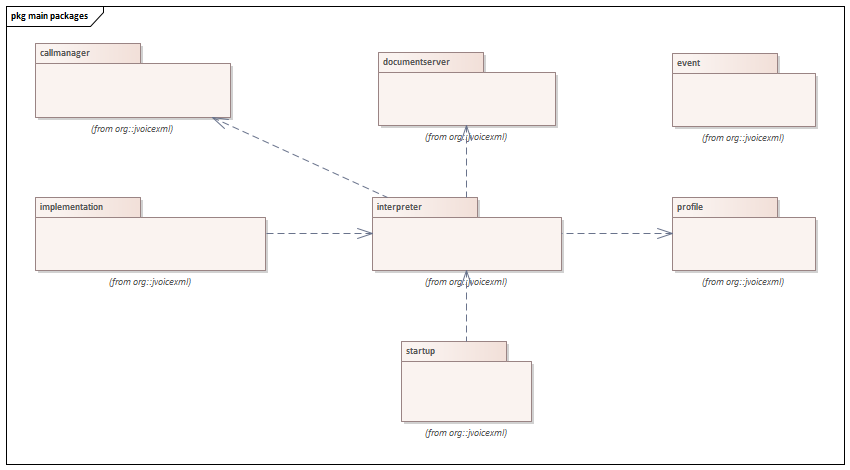
\includegraphics[width=\linewidth]{main-packages.png}
\caption{Main pacakages of JVoiceXML}
\label{fig:main-packages}
\end{figure}


Within a project the following directory structure applies

\begin{description}
\item[3rdparty] third party libraries. This directory contains all libraries
that are used by the specific project 
\item[classes] compiled binaries
\item[etc] resource files
\item[src] Java source code
\item[unittests] JUnit tests and other tests. The code is located within a
dedicated \texttt{src} subfolder. The binaries are built into the subfolder
\texttt{classes}.
\item[3rdparty-libs.xml] ANT setting for the third party libraries
\item[build.xml] main ANT build file for this project
\item[test.xml] ANT build file to to run the unit tests for this project.
\ref{sec:create-configuration})
\end{description}

Demo projects may have an additional folder \texttt{config} to hold
configurations settings. 

\section{JVoiceXML Core}
\label{sec:jvoicexml-core}

The core of JVoiceXML comprises the following sub-projects:

\begin{description}
\item[org.jvoicexml] The core of the interpreter (Required)
\item[org.jvoicexml.config] JVoiceXML configuration based on spring (Required)
\item[org.jvoicexml.client] Client libraries to interacti with JVoiceXML remotely. (Required)
\item[org.jvoicexml.client.text] Text client for the text based
implementation platform.
\item[org.jvoicexml.xml] The JVoiceXML XML library (Required)
\item[org.jvoicexml.jndi] JNDI support for JVoiceXML (Required)
\item[org.jvoicexml.processor.srgs] SRGS processor (Required)
\item[org.jvoicexml.callmanager.mmi] Demo implementation for the W3C MMI
architecture.
\item[org.jvoicexml.callmanager.mmi.umundo] Event and transport layer
based on umundo for \texttt{org.jvoicexml.callmanager.mmi}.
\item[org.jvoicexml.callmanager.mmi.socket] Event and transport layer
based on sockets for \texttt{org.jvoicexml.callmanager.mmi}.
\item[org.jvoicexml.callmanager.sip] Demo implementation for SIP based access to
JVoiceXML.
\item[org.jvoicexml.callmanager.text] Demo implementation for text based access to
JVoiceXML.
\item[org.jvoicexml.implementation.jsapi10] Demo implementation platform for
JSAPI 1.0~\cite{sun:jsapi}.
\item[org.jvoicexml.implementation.jsapi20] Demo implementation platform for
JSAPI 2.0~\cite{jcp:jsr113}.
\item[org.jvoicexml.implementation.jtapi] Demo implementation platform for
JTAPI 1.3~\cite{sun:jtapi}.
\item[org.jvoicexml.implementation.mary] Demo implementation platform for
the Mary Open TTS system.
\item[org.jvoicexml.implementation.marc] Demo implementation platform for
the MARC.
\item[org.jvoicexml.implementation.mrcpv2] Demo implementation platform for
MRCPv2.
\item[org.jvoicexml.implementation.text] Demo implementation platform for
text based access.
\item[org.jvoicexml.mmi.events] A library to author MMI events.
\end{description}

\subsection{Project \texttt{org.jvoicexml}}

This project is the core of the JVoiceXML browser and the central point of
building and configuring the environment.

\subsubsection{Directory Structure}
\label{sec:directory-structure}

Having the source code in your \$\{JVOICEXML\_HOME\}/org.jvoicexml
directory you find the following directory structure:

\begin{description}
\item[3rdparty] third party libraries. This directory contains all libraries
that are used by the core or by more that one subproject. Hence, it serves as a
central library repository. 
\item[classes] compiled binaries
\item[config] configuration setting to run the voice browser
\item[config-props] configuration templates for the ant build files
\item[dist] distribution files
\item[etc] resource files
\item[personal-props] adapted configuration from the configuration templates
for the ant build files. The contents of this folder is never committed to the
SVN repository except the \texttt{README.TXT}.
\item[logging] logging output of JVoiceXML
\item[src] Java source code
\item[unittests] JUnit tests and other tests
\item[work] Recorded audio files
\item[3rdparty-libs.xml] ANT setting for the third party libraries
\item[build.xml] main ANT build file
\item[configuration.xml] ANT build file to create a customized configuration
\item[distribution.xml] ANT build file to create the distribution
\item[nightly.xml] ANT build for the nightly build process
\item[run.xml] ANT build file to run the voice browser
\item[test.xml] ANT build file to to run the unit tests
\item[platform-targets.xml] Included ANT build file that will call the
configured implementation platforms (see sections \ref{sec:adapt-ant} and
\ref{sec:create-configuration})
\end{description}

Not all of the files are present at start but are created by the
ANT build file or through procedures described in this 
document, see section~\ref{sec:ant-build-file} or while running the interpreter.

\subsubsection{Adapting the ANT Configuration}
\label{sec:adapt-ant}

The directory \texttt{personal-props} provides a developer with the 
possibility to override some 
default properties defined by files in \texttt{config-props}. 
Any file that is to be
substituted must be copied from \texttt{config-props} 
(preserving the directory structure) to that directory and can then be 
modified. Do not modify the settings in the \texttt{config-props} folder. This
is a possible source for SVN conflicts.

The settings in the build.xml files assure that the files
found in this directory have precedence over those in config-props.

\subsubsection{Third Party Libraries}
\label{sec:third-party-libr}

JVoiceXML uses some third party libraries. This section names them and tell
you where you can get them. All of them are at least freeware
so that it was possible to store them in the SVN repository at
SourceForge. You can download them either from that location or
from their home pages. 

In this section, only those libraries are described, that are required
to build the main project. Some implementation platforms or demos may
require additional libraries.

You can also use your local copy by adjusting the settings in your
custom properties file. However, this is not recommended.

The settings of these libraries are stored in the file \emph{3rdparty-libs.xml}
which is imported by the main build file.

All third party libraries are located in the directory \\
\$\{JVOICEXML\_HOME\}/3rdparty.

This directory is assigned to the property \\
\texttt{3rdparty.dir}

Each library is located in a specific subfolder of the \$\{3rdparty.dir\}
folder. These subfolder follow this convention:

\begin{itemize}
\item The name of the subfolder is a combination of the library name and
the version of this library, e.g. \texttt{log4j1.2.17} for the \emph{log4j}
library with the version number\emph{1.2.16}.
\item The jars of this library are located in a subfolder of this folder
called \emph{lib}
\item The Javadoc documentation for the library is compressed into a zip
archive and added to the subfolder.
\end{itemize}

You find a copy of the license terms for the libraries in the folder\\
\$\{JVOICEXML\_HOME\}/etc/legal.

\paragraph{Library Snapshots}

Some of the used libraries are under active development and have not yet
released a patched release. In these cases the lib folder contains a snapshot
from their repository. The presence of a snapshot is marked in the file
\texttt{doc/libraries.xhtml} e.g. with the comment \emph{(SVN snapshot from
<date>)}.

\subsubsection{Libraries Needed to Compile JVoiceXML}
\label{sec:libr-need-comp}

\paragraph{log4j 1.2.17}

JVoiceXML uses log4j~\cite{apache:log4j} for logging. We think that log4j has 
some advantages
over \texttt{java.util.logging} and appears to be more mature and reliable.

The output of SUN's own logging framework can be redirected to log4j via the
system property
\begin{lstlisting}
-Djava.util.logging.config.file=${config}/logging.properties
\end{lstlisting}

This file contains the description of a logging handler that forwards all
request to log4j. Hence, both the log4j logging framework and SUN's logging
framework can be configured through the log4.xml configuration file.

\paragraph{Rhino 1.7R3}

JVoiceXML uses rhino~\cite{rhino} from Mozilla to enable scripting.
Java 6 already comes with a rhino implementation, but since we need to
build custom components we can not rely on this.

\paragraph{jsonsimple1.1}

Helps to parse JSON formatted JavaScript.

\paragraph{Commons pool 1.5.5}

The pooling of implementation platform resources is based on commons
pool.

\paragraph{Commons HTTP client 4.2.3}

The HTTP client library is used to retrieve VoiceXML documents from a web
server.

\paragraph{Commons HTTP core 4.2.3}

Core HTTP functionalities needed by the HTTP client.

\subsubsection{Libraries Needed at Run-time}

Besides the libraries named in section~\ref{sec:libr-need-comp} the following
libraries are needed to run JVoiceXML.

\paragraph{Commons Logging 1.1.1}
\label{sec:commons-logging}

This library is required by the other commons libraries.

\paragraph{Commons Codec 1.4}
\label{sec:commons-codec}

This library is required by the HTTP client to add attachments to the POST and
GET requests.


\subsubsection{Other Libraries}

Besides the libraries named above there are also other libraries in the
3rdparty folder. These libraries are used by more than one other implementation
platforms and are kept here as a general pool. Libraries that are used only by
one single implementation platform are located in the implementation platform's
3rdparty library directory.


\subsubsection{Creating a Configuration}
\label{sec:create-configuration}

Currently there are eleven implementations for the implementation platform
that reside in co-projects, refer to section~\ref{sec:svn-repository}.

Section~\ref{sec:adapt-ant} describes how to prepare your personal settings.
If you want to use one of them, you have to adapt the corresponding setting in
your copy of \texttt{platforms.xml} in the folder\texttt{personal-props} by
simply uncommenting it.
An example to enable the JSAPI 1.0 platform is shown below:
\begin{lstlisting}[language=XML]
<?xml version="1.0" encoding="UTF-8" standalone="yes" ?>
<platforms>
  <!--
     Uncomment the platforms that you want to use or add your own platform.
  -->
  <platform name="org.jvoicexml.implementation.jsapi10">
    <property name="jvxml.jsapi10.talkingJava" value ="false" />
    <property name="jvxml.jsapi10.talkingJava.path"
        value ="../org.jvoicexml.implementation.jsapi10/3rdparty/talkingjava/lib" />
  </platform>
  <!-- platform name="org.jvoicexml.implementation.jsapi20">
    <property name="jvxml.jsapi20.sapi" value ="false" />
    <property name="jvxml.jsapi20.mac" value ="false" />
  </platform-->
  <!-- platform name="org.jvoicexml.implementation.jtapi"/-->
  <!-- platform name="org.jvoicexml.implementation.mary"/-->
  <!-- platform name="org.jvoicexml.implementation.marc"/-->
  <!-- platform name="org.jvoicexml.implementation.mrcpv2"/-->
  <!-- platform name="org.jvoicexml.implementation.red5"/-->
  <!-- platform name="org.jvoicexml.callmanager.sip"/-->
  <!-- platform name="org.jvoicexml.callmanager.mmi">
    <subproject name="org.jvoicexml.mmi.events" order="pre" />
    <!-- For this platform to work you will need at least one of the
         following subprojects -->
    <!-- uncomment if MMI events should be handled over umundo -->
    <!-- subproject name="org.jvoicexml.callmanager.mmi.umundo"
        order="post" /-->
    <!-- uncomment if MMI events should be handled over sockets -->
    <!-- subproject name="org.jvoicexml.callmanager.mmi.socket"
        order="post" /-->
  </platform-->
  <!-- platform name="org.jvoicexml.callmanager.text"/-->
  <!-- platform name="org.jvoicexml.implementation.text"/-->
</platforms>
\end{lstlisting}

This will enable the JSAPI 1.0 platform to work with Sphinx 4 and FreeTTS. 

This setting is also used if you call ant for the main build file as described
in the following section.
Note that you need at least one implementation platform to use the voice
browser.

An implementation platform or callmanager is configured using the
\lstinline{platform}-tag. The name of the platform given via the
\lstinline{name} attribute must match the name of a project, i.e. the
platform or callmanager to configure.

A \lstinline{platform}-tag may contain nested ANT tags, e.g.
\lstinline{property}, which are copied into the resulting ANT build file. Moreover, a \lstinline{platform}-tag
may have nested \lstinline{subproject} tags. Its \lstinline{name} attribute
is used to identify subprojects that have to be compiled before
(\lstinline{order} set to \texttt{pre}) or after the platform project
(\lstinline{order} set to \texttt{post}). Again the value given at the
\lstinline{name} attribute must match the name of the project.

Once you changed the settings call
\begin{lstlisting}
ant -f configuration.xml
\end{lstlisting}
to create your adapted configuration settings. In addition you also get
a customized ant build file \texttt{run.xml} as well as the included
\texttt{platform-targets.xml} to start and
stop the interpreter using the libraries from the co-projects.
Eclipse users may want to read section~\ref{sec:ant-eclipse} if they do
not how hot wo run ANT build files from eclipse. 

Note that it is required to create a configuration after you changed the
settings in the \texttt{ant.properties} file.

The voice browser can be started by
\begin{lstlisting}
ant -f run.xml run
\end{lstlisting}
and stopped by
\begin{lstlisting}
ant -f run.xml shutdown
\end{lstlisting}

Please do not stop the voice browser by \texttt{CTRL-C} or similar. It may occur
that some resources are not closed properly and may cause conflicts with the next
start of JVoiceXML.

This target will try to determine the current SVN version number using JavaHL. On
windows systems this may cause some trouble. In case you encounter any problems,
please read the instructions at \url{http://subclipse.tigris.org/wiki/JavaHL}.

The created \texttt{run.xml} also contains a target to enable remote
debugging. It can be called by
\begin{lstlisting}
ant -f run.xml debug
\end{lstlisting}
The code will be compiled using your current configuration and the start of the
voice browser will be delayed until you connect with a remote debugger. The
used server port is 12367. This allows to set breakpoints using your IDE and
debug JVoiceXML.

\subsubsection{The Main Build File}
\label{sec:ant-build-file}

This section explains the most important targets of the main build file
\texttt{build.xml}. All others buildfiles from the implementation platforms
are called from this central point. Just start ant without any target specified
if you want to build everything. Call
\begin{lstlisting}
ant -projecthelp
\end{lstlisting}
to get an overview of the targets and their purpose.

Some of the targets use third party extensions to ANT. These 
extensions are not described in this document, but are part of
the 3rdparty folder. In contrast to the libraries to link with,
these libraries are not defined in the file \texttt{3rdparty-libs.xml}
but in the corresponding target of this build file. Each features
a preceding target that checks if the library is required. If
the library is not found, the target will not be called.

\begin{description}
\item[clean]
Delete all compiled class files in the directory \emph{classes}
and the jars that are created by the \emph{jar} target in the directory 
\emph{dist}.

\item[compile]
 Compile all JAVA files in the directory \emph{src} into the directory
\emph{classes}.

\item[jar]
 This target depends on the target \emph{compile} and creates the jar
files of your distribution in the directory \emph{dist}.
If successful, you will find at minimum the following jar archives:
\begin{itemize}
\item jvxml.jar This jar file contains the core of JVoiceXML.
\item jvxml-xml.jar This jar contains all files that are required
to create and parse VoiceXML documents. This file is being build from the
project \texttt{org.jvoicexml.xml} which is described in
section~\ref{sec:org.jvoicexml.xml}.
\item jvxml-client.jar This jar contains the files needed to build
a client.
\item jvxml-jndi.jar JNDI support for JVoiceXML
\item some other jars, depending on your configuration settings
\end{itemize}

\item[apidoc]
Create JAVADOC documentation from the JAVA files in the directory
doc/api.
\item[checkstyle]
Perform a check of the JVoiceXML coding standard as specified 
in section~\ref{sec:code-conventions}.
\end{description}

Call
\begin{lstlisting}
ant <target>
\end{lstlisting}
to run ant for the the given target.

The ANT launch configurations for eclipse are part of the SVN repository. They
are available as a shortcut in the external tools configuration after a first
run. A screenshot is shown in figure~\ref{fig:eclipse-launch}.
\begin{figure}
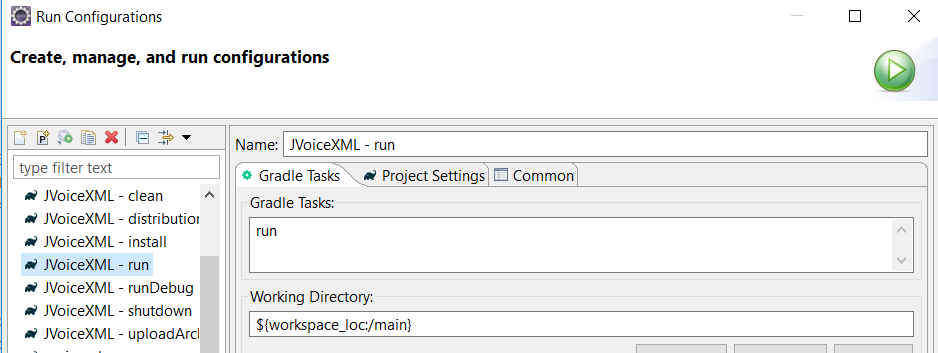
\includegraphics[width=\linewidth]{eclipse-launch.png}
\caption{Eclipse External Tools Configuration for JVoiceXML}
\label{fig:eclipse-launch}
\end{figure}

In some cases you will see some warnings when executing the
\lstinline{-version} target. Usually, these warnings can be ignored. In order
to get rid of it, you will have to ensure that \lstinline{svn} (or
\lstinline{svn.exe} for Windows systems) can be found on the OS's path. Usually
this is not the case if you are using Tortoise on Windows. Therefore, you will
have to donwload and install it separately from
\url{http://subversion.apache.org/packages.html}.

\subsection{Project \texttt{org.jvoicexml.config}}
\label{sec:org.jvoicexml.config}

This project provides a library to configure JVoiceXML based on the spring
framework.
This is not required at run time and can be replaced by custom
implementations, e.g. to embed JVoiceXML. However, it is required to build
JVoiceXML.

This project has to be build after the main project.

\subsubsection{Third party libraries}
\label{sec:config-third-party-libr}

\paragraph{Spring Framework 3.2.1}
\label{sec:spring-framework}

JVoiceXML uses the spring framework to address configuration issues.

\subsection{Project \texttt{org.jvoicexml.xml}}
\label{sec:org.jvoicexml.xml}

This project provides an XML library to create and parse all VoiceXML related
XML languages like SRGSXML, PLS and SSML.

This project has to be build before the main project.

\subsection{Project \texttt{org.jvoicexml.processor.srgs}}
\label{sec:org.jvoicexml.processor.srgs}

This project provides an SRGS processor.

This project has to be build before the main project.

\section{Remote Java Applications}
\subsection{Project \texttt{org.jvoicexml.client}}

This project contains the basic classes that are needed to implement a
client that can connect remotely to JVoiceXML.

\subsubsection{Third party libraries}

This platform makes use of the \lstinline{org.jvoicexml.jndi} library
to connect to JVoiceXML (see section\ref{sec:jndi}). In addition specialized
libraries from the implementation platform (see section
\ref{sec:implementation-platforms}) maybe required.

\subsection{Project \texttt{org.jvoicexml.jndi}}
\label{sec:jndi}

This project provides JNDI support for JVoiceXML. This is not required at run
time but in order to build JVoiceXML.

JNDI offers remote access to JVoiceXML, e.g. the ability to run the
shutdown script or to run the demos.

The project settings for this subproject can be adapted by the following ANT
properties in your copy of the \texttt{ant.properties} file in the
\texttt{personal-props} folder of the core project (see 
section~\ref{sec:adapt-ant}):
\begin{lstlisting}
jvxml.jndi.repository=text
jvxml.jndi.port=1099
\end{lstlisting}

The configuration ANT script also adapts the settings in the
\texttt{jndi.properties} to the configured port. Make sure to also adapt
the \texttt{jndi.properties} in the demos or your application.

The repository entry must match the repository that you are using for your
client. Otherwise JVoiceXML will not be able to load the needed resources of
the server side.

\section{Implementation Platforms}
\label{sec:implementation-platforms}

\subsection{JSAPI 10 Implementation Platform}
\label{sec:implementation-jsapi10}

\subsubsection{Project \texttt{org.jvoicexml.implementation.jsapi10}}

This project provides an implementation platform for JSAPI 1.0 compliant
speech engines. Besides a general hook for those engines there are also
extensions for FreeTTS and Sphinx 4 bases on these hooks to demonstrate the
capabilities.

The project settings for this subproject can be adapted by the following
properties in the \texttt{platforms.xml}

\begin{description}
\item[jvxml.jsapi10.talkingJava] A value of \texttt{false} will result in a
configuration that uses FreeTTS and Sphinx4 as speech engines. If set to
\texttt{true} the Talking Java wrapper for Microsoft's speech engine will be
used. In the latter case you need also to specifiy a value for
\texttt{jvxml.jsapi10.talkingJava.path}
\item[jvxml.jsapi10.talkingJava.path] A path that is used to locate the DLLs
that are required to use Talking Java as sthe speech engine.
\end{description}

\subsubsection{Third party libraries}
\label{sec:jsapi10-third-party-libr}

\paragraph{JSAPI 1.0}

This library contains the Java Speech API v1.0
(JSAPI)~\cite{sun:jsapi} to address speech recognition and speech synthesis
issues. It is a pure API layer without any concrete TTS or ASR implementations
which have to be added in addition.


\paragraph{FreeTTS 1.2.2}
\label{sec:freetts}

JVoiceXML uses FreeTTS~\cite{freetts} as a demo implementation for TTS output.
FreeTTS comes with two libraries: One for the general functionality
and one custom for the JSAPI 1.0 support.
The general library is kept in the core project's 3rdparty library directory
and the JSAPI library can be found in this project's 3rdparty library directory.

Note that the used library is a snapshot from the FreeTTS SVN repository.

\paragraph{CMU sphinx 4}
\label{sec:sphinx}

JVoiceXML uses sphinx 4~\cite{sphinx} from Carnegie Mellon University
as a demo implementation for speech recognition.

Note that the used library is a snapshot from the sphinx SVN repository.

\paragraph{Talking Java}

Talking Java is an implementation of the JSAPI 1.0 utilizing Microsoft's
SAPI4 and SAPI5 speech engines. It can be used as a replacement for FreeTTS
and CMU sphinx4. Note that the delivered version is only free for personal use.
If you intend to use it in a commercial corporate or institutional context, you
will have to buy a license. Please refer to \url{http://www.cloudgarden.com}.

\subsection{JSAPI 2.0 Implementation Platform}
\subsubsection{Project \texttt{org.jvoicexml.implementation.jsapi20}}

This project contains a first draft of an implementation platform to enable
JSAPI 2.0 support for JVoiceXML.

This implementation platform makes use of the reference implementation (RI) that
can be obtained from Conversay web page
conversations~\cite{conversay:jsr113}. Note that this is not the final release
but the release candidate. It will not run on embedded devices since it makes
use of Conversay's speech engine that is only compatible with the Windows
operating system.

\subsubsection{Third party libraries}
\label{sec:jsapi20-third-party-libr}

\paragraph{JSAPI 2.0}
\label{sec:jsapi20}

The JSAPI 2.0 specification is under going changes.
JSAPI 2.0 is being developed within
the Java Community Process (JCP)~\cite{jcp} under 
JSR-113~\cite{jcp:jsr113}.

This open source library library provides a framework to ease the development of
JSAPI 2.0 compliant speech engines. The project also provides custom extensions for
FreeTTS and sphinx. The project URL is \url{http://jsapi.sourceforge.net}.

Note that the used library is a snapshot from the jsapi SVN repository.

\paragraph{jlibrtp 0.2}

jlibrtp is used to enable streaming of audio data via the RTP protocol.This
is being used to stream the audio coming from the JSAPI 2.0 compliant
engines to the client. The project URL is \url{http://jlibrtp.sourceforge.net}.

Note that the used library is a snapshot from the jlibrtp SVN repository.

\paragraph{FreeTTS 1.2.2}

The JSAPI 2.0 implementation platform uses the general library from
FreeTTS~\cite{freetts} as a demo implementation for TTS output.

Note that the used library is a snapshot from the FreeTTS SVN repository.

\paragraph{CMU sphinx 4}
\label{sec:sphinx}

The JSAPI 2.0 implementation platform uses sphinx 4~\cite{sphinx} from
Carnegie Mellon University as a demo implementation for speech recognition.

\subsection{JTAPI 1.3 Implementation Platform}
\subsubsection{Project \texttt{org.jvoicexml.implementation.jtapi}}

This implementation platform provides telephony functionality based on JTAPI to
JVoiceXML.This implementation platform should be used together with other
implementation platforms like the JSAPI 2.0 implementation platform since it
does not have any speech functionality.

The project settings for this subproject can be adapted by the following ANT
properties in your copy of the \texttt{ant.properties} file in the
\texttt{personal-props} folder of the core project (see 
section~\ref{sec:adapt-ant}):
\begin{lstlisting}
jtapi.sip.providername=net.sourceforge.gjtapi.raw.mjsip.MjSipProvider
jtapi.sip.address=127.0.0.1:4242
jtapi.sip.terminal = sip:jvoicexml@127.0.0.1:4242
jtapi.sip.port=4242
jtapi.sip.inputType=jsapi20
jtapi.sip.outputType=jsapi20
\end{lstlisting}

\subsubsection{Third party libraries}
\label{sec:jtapi-third-party-libr}

\paragraph{JTAPI 1.3}

JTAPI is used to address telephony issues.

\paragraph{GJTAPI 1.9RC2}

GJTAPI is used to simply the use of the JTAPI layer. Besides the core library
we use the mjsip provider from this project.

Note that the used library is a modified version. Modifications include
\begin{itemize}
\item bug fixes of the SIP provider
\end{itemize}

\paragraph{mjsip}

MjSIP provides an easy way to have SIP functionality. Unfortunately, this
project uses the GPL license which makes is unusable in commercial
applications. It should be replaced by JainSIP.

\subsection{MARC implementation Platform}
\subsubsection{Project \texttt{org.jvoicexml.implementation.marc}}

This implementation integrates MARC system into JVoiceXML. This platform
only provides the output part and is designed to be used with other
implementation platforms like JSAPI 1.0, see section~\ref{sec:implementation-jsapi10}.

Note that you will need a MARC instance running if you want to use this
demo. MARC can be downloaded from \url{http://marc.limsi.fr/}.

This implementation platform will allow for the integration of MARC BML commands
into your VoiceXML files.

\subsection{OpenMary Implementation Platform}
\subsubsection{Project \texttt{org.jvoicexml.implementation.mary}}

This implementation integrates the Mary TTS system into JVoiceXML. It is
designed to be used with other implementation platforms like JSAPI 1.0, see
section~\ref{sec:implementation-jsapi10}.

Note that you will need a Mary 4.0.0  TTS server running if you want to use this
demo. Mary has to be configured as a socket server, therefore edit and file
\texttt{MARY\_HOME/conf/marybase.config} and change the following line 

\begin{lstlisting}
# Type of server? (socket/http/commandline)
server = http
\end{lstlisting}

to

\begin{lstlisting}
# Type of server? (socket/http/commandline)
server = socket
\end{lstlisting}

\subsubsection{Third party libraries}
\label{sec:mary-third-party-libr}

\paragraph{Mary client}

The Mary client is shipped with the Mary TTS systems and facilitates the
communication of clients like JVoiceXML with the Mary TTS server.

\subsection{MRCPv2 Implementation Platform}

\subsubsection{Project \texttt{org.jvoicexml.implementation.mrcpv2}}

This implementation platform aims at MRCPv2 support for JVoiceXML. It is in the
starting phase and currently it is not usable.

This implementation platform requires the presence of an MRCPv2 server. An open
source solution based on FreeTTS and sphinx 4 can be downloaded from
\url{http://cairo.sourceforge.net}.

To make use of this implementation platform, JVoiceXML must be called with a SIP
phone. We used the xlite phone which can be downloaded for free from
\url{http://www.counterpath.com}.

The project settings for this subproject can be adapted by the following ANT
properties in your copy of the \texttt{ant.properties} file in the
\texttt{personal-props} folder of the core project (see 
section~\ref{sec:adapt-ant}):
\begin{lstlisting}
mrcpv2.sip.address=127.0.0.1:4242
mrcpv2.sip.port=4242
mrcpv2.sip.cairo.sip.address=sip:cairo@speechforge.org
mrcpv2.sip.cairo.sip.host=127.0.0.1
mrcpv2.sip.cairo.sip.port=5050
\end{lstlisting}

\subsubsection{Third party libraries}
\label{sec:mrcpv2-third-party-libr}

\paragraph{mrcp4j}

Mrcp4j provides the core functionality for the MRCPv2 integration.

\paragraph{Cairo}

Cairo is required as a means for communication with MRCPv2 resources.

\subsection{Project \texttt{org.jvoicexml.implementation.text}}

The text based implementation platform provides a text based input and output.
This means that you receive the system output as Java strings and you are able
to provide input via Java strings.

\subsubsection{Third party libraries}
\label{sec:text-third-party-libr}

No special libraries.

\subsection{MMI CallManager}
\subsection{Project \texttt{org.jvoicexml.callmanger.mmi}}

This callmanager allows for accessing JVoiceXML as a modality component in
the W3C MMI architectural pattern~\cite{w3c:2012:mmi_arch}.

\subsubsection{Third party libraries}

This platform makes use of the \lstinline{org.jvoicexml.mmi.event} library
to author MMI compatible events (see section~\ref{sec:mmi-events}).
Support for VoiceXML snippets is gained by the use of the MMI Servlet
(see section~\ref{sec:mmi-servlet}).
In addition an implemention of an Event and Transport Layer is needed.

\subsection{Project \texttt{org.jvoicexml.mmi.socket}}

This project contains an implementation of the Event and Transport Layer
via sockets. MMI events are received as XML.

\subsubsection{Third party libraries}

This platform makes use of the \lstinline{org.jvoicexml.mmi.event} library
to author MMI compatible events (see section\ref{sec:mmi-events}).

\subsection{Project \texttt{org.jvoicexml.mmi.umundo}}

This project contains an implementation of the Event and Transport Layer
via umundo\footnote{\url{https://github.com/tklab-tud/umundo}}.
MMI events are received as protopuf messages.

\subsubsection{Third party libraries}

\paragraph{protobuf2.5.0}

Needed for MMI generation in Google's protobuf format.

\subsection{Project \texttt{org.jvoicexml.callmanager.mmi.servlet}}
\label{sec:mmi-servlet}

This project adds support for VoiceXML snippets that can be received
in the \lstinline{Content} attributes of the \lstinline{PrepareRequest}
or \lstinline{StartRequest} of the MMI events.

The resulting web archive must be deployed manually to a servlet container
of your choice (see section \ref{sec:tomcat}).

\subsubsection{Third party libraries}

\paragraph{servlet API}

Servlet API needed for the Servlets.

\subsection{Project \texttt{org.jvoicexml.mmi.events}}
\label{sec:mmi-events}

This project is a library to author MMI compatible events that can be used in
the MMI architectural pattern from the W3C.

Currently the library is able to generate events in XML format and for
protobuf~\cite{google:protobuf}. The generation of Java files for protobuf
support requires the download of the \texttt{protoc} compiler. The \texttt{protoc}
executable can be downloaded from \url{http://code.google.com/p/protobuf/downloads/list}.

The project settings for this subproject can be adapted by the following ANT
properties in your copy of the \texttt{ant.properties} file in the
\texttt{personal-props} folder of the core project (see 
section~\ref{sec:adapt-ant}):
\begin{lstlisting}
mmi.protoc=protoc
\end{lstlisting}

\subsubsection{Third party libraries}

\paragraph{protobuf2.4.1}

Needed for MMI generation in Google's protobuf format.

\subsection{SIP Implemetation Platform}
\subsubsection{Project \texttt{org.jvoicexml.callmanger.sip}}

This callmanager aims at supporting SIP based access to JVoiceXML.

\subsubsection{Third party libraries}

\paragraph{jainsip1.2}

JainSIP provides a SIP stack for Java.

\subsection{Text Implementation Platform}
\subsubsection{Project \texttt{org.jvoicexml.callmanger.text}}

This callmanager aims at accesssing JVoiceXML as a server for text based
access. In contrast to the text based implementation platform this callmanager
doese not require JNDI.

\subsubsection{Third party libraries}

No special libraries.



\section{Demo Programs}

The demo programs give a short impression how the JVoiceXML voice browser can
be used.

The demos comprise the following sub-projects:

\begin{description}
\item[org.jvoicexml,demo.embedded] A demo project that shows how JVoiceXML can
be embedded into other projects.
\item[org.jvoicexml,demo.helloworlddemo] The venerable hello world in Voice\-XML
\item[org.jvoicexml.demo.helloworldservletdemo] The same but as a servlet
\item[org.jvoicexml.demo.inputdemo] A small cinema application
\item[org.jvoicexml.demo.jtapidemo] SIP based access to JVoiceXML calling the
hello world servlet demo (not functional)
\item[org.jvoicexml.demo.marcdemo] Demo to show how the interaction with MARC.
\item[org.jvoicexml.demo.mixedinitiativedemo] Demo to show how the mix\-ed
initiative capabilities.
\item[org.jvoicexml.demo.objecttagdemo] Demo to show how the object tag can be
used.
\item[org.jvoicexml.demo.recorddemo] Demo for the record tag
\item[org.jvoicexml.demo.scriptdemo] Demo for scripting functionality with a
weird dialog flow
\item[org.jvoicexml.demo.subdialogdemo] Demo to show a subdialog
\item[org.jvoicexml.demo.textdemo] Demo to show how to use the text platform
\item[org.jvoicexml.demo.voicexmlcreationdemo] Demo for the VoiceXML XML library
\end{description}

\section{Eclipse Plug in}

The eclipse plug-in allows to run JVoiceXML as a server from within the eclipse
IDE.

\begin{description}
\item[org.jvoicexml.eclipse.jst.server] Eclipse plug-in to start the JVoiceXML
from the eclipse server view.
\item[org.jvoicexml.eclipse.features] Eclipse features for the JVoiceXML
plug-in.
\item[org.jvoicexml.eclipse.updatesite] Eclipse update site for the
JVoiceXML plug-in
\end{description}

\section{VoiceXML Unit}
\section{voicexml-unit}

This component is an approach to establish unit testing capabilities for
VoiceXML.

\section{System test}

The system test implements the W3C's conformance test for VoiceXML 2.1.

\begin{description}
\item[org.jvoicexml.voicexmlunit] VoiceXML unit test framewortk
\item[org.jvoicexml.voicexmlunit] Demo test project
\end{description}

In addition you will need the following sub-projects:
\begin{itemize}
\item org.jvoicexml
\item org.jvoicexml.xml
\item org.jvoicexml.implementation.text
\end{itemize} 

\section{Documentation}

JVoiceXML documentation as \LaTeX files.

The documentation comprise the following sub-projects:

\begin{description}
\item[extensionguide] The extension guide for JVoiceXML
\item[howtobuild] The how to build JVoiceXML documentation (this document)
\item[htdocs] The HTML web pages
\item[userguide] A tutorial to start working with JVoiceXML
\end{description}

\section{Code Conventions}
\label{sec:code-conventions}

We follow the JAVA code conventions~\cite{sun:codeconv} for our code. All
methods and member variables must be commented using 
JAVADOC~\cite{sun:javadoc_guidelines}.

In addition we use a custom \texttt[language=Java]{@todo} JAVADOC tag or a
\texttt{TODO} tag to mark sections that need further work.

Example:

\begin{lstlisting}[language=Java]
/** @todo Implement the untreated case XYZ */
\end{lstlisting}

We use checkstyle~\cite{checkstyle} to check our coding conventions.
All developers are requested to execute the \emph{checkstyle} target
of our ANT buildfile, see section~\ref{sec:ant-build-file}. 
There are plug-ins for some IDEs, which you can use if you want to. The
\texttt{checkstyle.xml} can be found in the folder 
\texttt{etc} and is called \texttt{jvoicexml-checks.xml}.

With the help of the checkstyle plugin these tests can be run automatically
and visualized inside eclipse. Therefore, each project has to be configured to
use this project relative configuration file. A screenshot is shown inside
figure~\ref{fig:eclipse-project-checkstyle}.
\begin{figure}
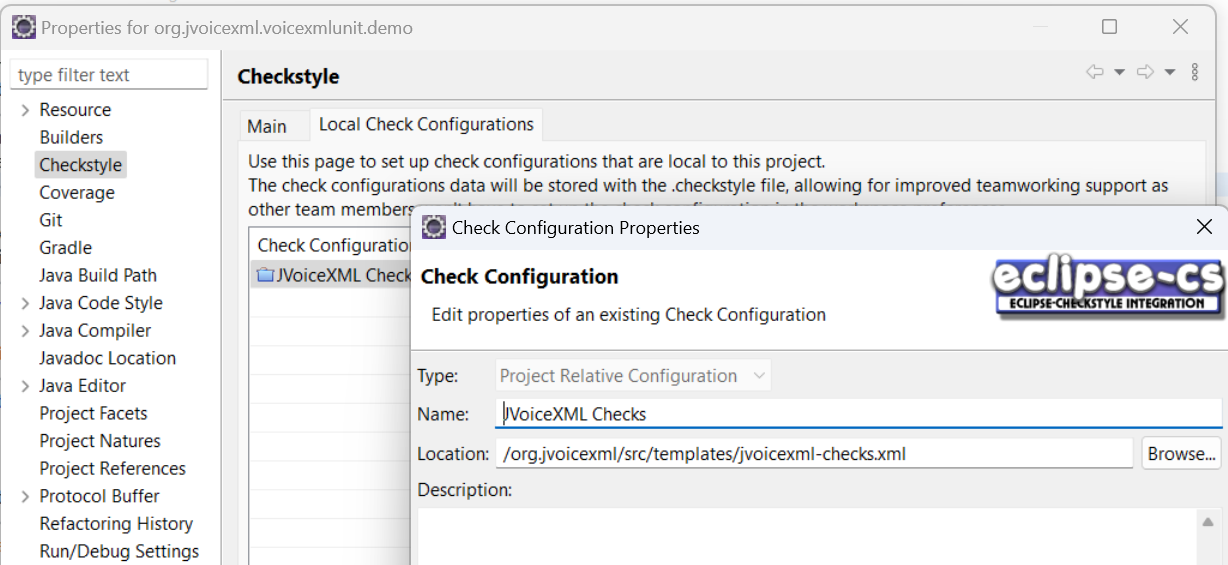
\includegraphics[width=\linewidth]{eclipse-project-checkstyle.png}
\caption{Project relative configuration of checkstyle within eclipse}
\label{fig:eclipse-project-checkstyle}
\end{figure}


Developers are requested to use the \texttt[language=Java]{@inheritDoc}
JAVADOC tag in favor of a \texttt[language=Java]{@see} reference for inherited documentation.
Pros of the \texttt[language=Java]{@inheritDoc} tag, taken 
from~\cite{tauber:inheritdoc}, are
\begin{itemize}
\item satisfies checkstyle requirements for JAVADOC,
\item no references to go stale,
\item additional doc specific to this implementation will appear in JAVADOC and
\item inherited doc in JAVADOC.
\end{itemize}

All source files must contain the following header about the 
copyright, see section~\ref{sec:copyright}, that we use for JVoiceXML.

\begin{lstlisting}[language=Java]
/*
 * File:    $HeadURL: $
 * Version: $LastChangedRevision: $
 * Date:    $Date: $
 * Author:  $LastChangedBy: $
 *
 * JVoiceXML - A free VoiceXML implementation.
 *
 * Copyright (C) 2012 JVoiceXML group - 
 *      http://jvoicexml.sourceforge.net
 *
 * This library is free software; you can redistribute it 
 * and/or modify it under the terms of the GNU Library 
 * General Public License as published by the Free Software 
 * Foundation; either version 2 of the License, or (at your 
 * option) any later version.
 *
 * This library is distributed in the hope that it will be 
 * useful, but WITHOUT ANY WARRANTY; without even the 
 * implied warranty of MERCHANTABILITY or FITNESS FOR A 
 * PARTICULAR PURPOSE.  See the GNU Library General Public 
 * License for more details.
 *
 * You should have received a copy of the GNU Library 
 * General Public License along with this library; if 
 * not, write to  the Free Software Foundation, Inc., 
 * 59 Temple Place, Suite 330, Boston, MA  02111-1307  USA
 *
 */
\end{lstlisting}

The keywords embarrassed by \texttt{\$} are to be expanded by 
subversion. 
This means that for any \texttt{svn commit} the subversion
option \texttt{svn:keywords} has to be set by

\begin{lstlisting}
svn propset svn:keywords "HeadURL LastChangedRevision \
LastChangedDate LastChangedBy" <filename>
\end{lstlisting}.

Since this has to be done for each file, you might want to have a look
at the SVN's automatic property setting capability.

In order to activate it, locate the \texttt{config} file in you subversion home
folder and open it for editing. Under Linux you will usually find this
configuration folder \texttt{.subversion} in your home directory.

In the section \texttt{[miscellany]} set
\begin{lstlisting}
enable-auto-props = yes
\end{lstlisting}

In the section \texttt{[auto-props]} set
\begin{lstlisting}
*.java = svn:mime-type=text/plain;svn:eol-style=native;svn:\
keywords=Rev Date HeadURL LastChangedRevision LastChangedBy \
LastChangedDate
\end{lstlisting}

The class comment has to contain the following information:

\begin{lstlisting}[language=Java]

/**
 * Comment about the purpose of this class.
 *
 * @author <Name of the author>
 * @author <Other authors>
 *
 * @version $LastChangedRevision$
 * @since <current version number>
 */
\end{lstlisting}

Again the keyword expansion from subversion is used to expand the keyword,
\texttt{\$LastChangedRevision \$} in this case. The name of the author and the 
purpose have to be replaced by their proper values.

\section{Releases}

This section describes the required steps to create a new release for
JVoice\-XML.

\subsection{Creation of a Release Workspace}

New releases are \emph{never} built from the workspace to ensure that there are
no changes in the workspace that are not reflected in the SVN repository.
Therefore change to an empty directory and copy the following files from the
\texttt{org.jvoicexml} project to this new folder:
\begin{enumerate}
  \item nightly.xml
  \item all jars from the \texttt{3rdparty/svnant/lib} folder
\end{enumerate}
Open a command prompt at this directory and call
\begin{lstlisting}
ant -f nightly.xml checkout
\end{lstlisting}

The next step is to adjust you local settings. This can easily be done by
copying the contents of the personal-props directory of your development copy
of JVoiceXML to the personal-props directory of the new copy.


\subsection{Unit Tests}

There are many unit tests based on JUnit to ensure the correctness of the
classes written for JVoiceXML. Some tests need customized settings, e.g. to
start the Mary TTS server. These settings are maintained in the file
\texttt{config-props/test.properties} and can be overridden with a
personalized copy in the folder \texttt{personal-props}.

The unit tests are started from the core project
\texttt{org.jvoicexml}. It is the entry point of the unit tests of the various subproject. Therefore, change to the core directory of the release copy and call
\begin{lstlisting}
cd org.jvoicexml
ant -f nightly.xml unittests
\end{lstlisting}
This will take some time. The results of the unit tests of all sub-projects can
be viewed using your favorite web browser by opening
\texttt{org.jvoicexml/dist/unittests/html/index.html} after the tests are
finished. There must not be any errors or failures in the summary. Note that
some tests require an active Internet connection. 

If you detect any errors correct identify the cause for it, correct them
yourself or contact the responsible developer of the module. After the errors
have been fixed, restart from the beginning to make a new release.

\subsection{Create the Distribution}

After the unit test ran successfully, the binary distribution can be built. The
ANT script \texttt{distribution.xml} contains the needed targets.
Update the version number in the file \texttt{config-props/ant.properties}
and comment the version number in the copy in the folder
\texttt{personal-props}. The JVoiceXML version number consists of
\begin{lstlisting}
 <major-version>.<minor-version>.<bug-fix-level>.<EA|GA>
\end{lstlisting}
\textbf{E}arly \textbf{A}ccess (EA) versions are intended for intermediate
versions while \textbf{G}eneral \textbf{A}vailability (GA) versions are the
main versions that are available for download via the SourceForge file
downloads.

Create a distribution configuration by calling
\begin{lstlisting}
ant -f configuration createDistributionConfiguration
\end{lstlisting}

Call
\begin{lstlisting}
ant -f distribution.xml
\end{lstlisting}
to create the release. Make sure that the Javadoc output does not show any
errors. In case there are errors, correct them and repeat the creation of the
distributable.

All intermediate files are stored in the folder \texttt{dist/version}. The
distributable can be found in the folder of the core project after the
executing the ANT target.

\subsection{Test the Installation}

Run the installer to install the created distribution.
\begin{lstlisting}
java -jar jvxml-install-<version>.jar
\end{lstlisting}
Select all available packages and test the installation. 
Copy the jsapi2.jar to the lib folder of the installed version.
Start the voice browser and check if there are any errors in the log when
JVoiceXML starts.

Uninstall JVoiceXML and reinstall it with the JSAPI 1.0 implementation platform
only and the demos. Start JVoiceXML and check if all demos are working properly.
It should not be necessary to restart JVoiceXML while the demos are tested.

If any error occurs while testing, locate the cause of the error, fix it
yourself or identify the person who is responsible for the module and restart
the release process from the beginning.

\subsection{Tag the Release}

Commit the ANT properties file with the new version number.

The next step serves to tag the code of the release version. Therefore, you
will have to supply values for the properties
\begin{lstlisting}
svn.username=
svn.password=
\end{lstlisting}
in the ANT properties in the folder \texttt{personal-props}.

Call
\begin{lstlisting}
ant -f distribution.xml tag
\end{lstlisting}
to create copies of the source code in the SVN folder
\begin{lstlisting}
.../<subproject>/tags/<version>
\end{lstlisting}

\subsection{Upload the Distribution}

The upload comprises two parts:
\begin{enumerate}
  \item Javadoc upload
  \item Release upload
\end{enumerate}

Uploading requires the following properties in your personal copy of the ANT
properties:
\begin{lstlisting}
nightly.sf.user=
nightly.sf.password=
\end{lstlisting}

In order to upload the Javadoc, you first have to create the
destination folder at SourceForge. The name of the folder is
\begin{lstlisting}
/home/groups/j/jv/jvoicexml/htdocs/api/<version>
\end{lstlisting}
Make sure that the group can write the new folder and that other can access it.
The generated documentation can be copied by executing
\begin{lstlisting}
ant -f distribution.xml uploadJavadoc
\end{lstlisting}

The release is uploaded by 
\begin{lstlisting}
ant -f distribution.xml upload
\end{lstlisting}

\subsection{Update of the Website}

The web site needs some adaption to point to the new release when users click
on the download link. The download links can be found at the page
\texttt{downloads.html} in the project \texttt{htdocs}. Update the link
to the new release and commit the changes.

\subsection{Prepare the Further Development}

Prepare the next version by incrementing th version number in the ANT
properties file in the folder \texttt{config-props} and committing that file.

\subsection{Creation of Snapshots for Maven}

Some subprojects are ready to be upload snapshots for Maven to
Sonatype\footnote{\url{http://www.sonatype.com}}. Sonatype offers
a free repository hosting service using Nexus for open soource projects.

Therefore deployers are requested to sign up for their servie. Detailed
instructions are given at \url{https://docs.sonatype.org/display/Repository/Sonatype+OSS+Maven+Repository+Usage+Guide}.

Create the file \texttt{settings.xml} in the \texttt{.m2} folder in your
home directory with the following contents:

\begin{lstlisting}[language=XML]
<settings xmlns="http://maven.apache.org/SETTINGS/1.0.0"
        xmlns:xsi="http://www.w3.org/2001/XMLSchema-instance"
        xsi:schemaLocation="http://maven.apache.org/SETTINGS/1.0.0
         http://maven.apache.org/xsd/settings-1.0.0.xsd">>
  <servers>
    <server>
      <id>sonatype-nexus-snapshots</id>
      <username>your user name</username>
      <password>your password</password>
    </server>
    <server>
      <id>sonatype-nexus-staging</id>
      <username>your user name</username>
      <password>your password</password>
    </server>
  </servers>
</settings>
\end{lstlisting}

Insert your user name and your password at the marked entries.
Aftwerwards call 
\begin{lstlisting}
ant -f distribution.xml dist-maven-snapshot
\end{lstlisting}
in the core project \lstinline{org.jvoicexml}.

The snapshots will use the SVN version number to differntiate between different
snapshots of the same jar. Consequently, you will have to have at least
a commit between two snapshots.
\bibliography{howtobuild}
\bibliographystyle{plain}


\end{document}

% LocalWords:  JVoiceXML VoiceXML APIs JSAPI JTAPI mkdir cd CVS SourceForge cvs
% LocalWords:  pserver CVSROOT acls RSH lll xml LGPL src api JAVADOC rdparty XP
% LocalWords:  IDE jvoicexml dir JCP JSR jsapi BCL chmod FreeTTS TTS freetts
% LocalWords:  jvxml impl todo XYZ checkstyle Schnelle howtobuild basicstyle
% LocalWords:  RFE numberstyle stepnumber kkv href Revison JVoice Adrindam Das
% LocalWords:  TortoiseCVS cygwin  CMU tex schnelle WSJ gau dCep mel Mozilla
% LocalWords:  projecthelp backgroundcolor lightgray subfolder lang buildfile
% LocalWords:  plugins IDEs inheritDoc inhe rit RCSfile login apidoc loggings
% LocalWords:  distributionFolder IDE's Ingimar SVN svn trunc HTTPS config RTP
% LocalWords:  CLASSPATH GJTAPI jlibrtp JainSIP gjtapi HeadURL LastChangedDate
% LocalWords:  LastChangedRevision LastChangedBy propset
